\documentclass[aspectratio=169]{beamer}
% PhyriadFG — Estructura nueva + dependencias y conexiones
% Self-contained Beamer deck. Compile: pdflatex (TeX Live / MiKTeX), run twice.
% Mainstream packages only.
\usepackage[utf8]{inputenc}
\usepackage[T1]{fontenc}
\usepackage{xcolor}
\usepackage{booktabs}
\usepackage{longtable}
\usepackage{tikz}
\usetikzlibrary{arrows.meta,positioning,fit,backgrounds}

\usecolortheme{seahorse}
\setbeamertemplate{navigation symbols}{}
\setbeamertemplate{caption}{\insertcaption}
\setbeamerfont{frametitle}{size=\large}

% ---- per-layer colors (one per layer, reused consistently) ----
\definecolor{cliCol}{RGB}{70,110,180}   % CLI   (steel blue)
\definecolor{coreCol}{RGB}{200,120,30}  % CORE  (amber hub)
\definecolor{capCol}{RGB}{45,150,90}    % CAPTURE (green)
\definecolor{flowCol}{RGB}{30,160,170}  % FLOW  (teal)
\definecolor{warpCol}{RGB}{140,80,170}  % WARP/BLEND (purple)
\definecolor{presCol}{RGB}{205,70,70}   % PRESENT (red)
\definecolor{instCol}{RGB}{120,120,120} % INSTRUMENT (gray)
\definecolor{fwCol}{RGB}{75,90,115}     % FRAMEWORK (slate)
\definecolor{shCol}{RGB}{150,110,55}    % SHADERS (olive/brown)

\newcommand{\arr}{\ensuremath{\rightarrow}}
\newcommand{\barr}{\ensuremath{\leftrightarrow}}
\newcommand{\Lcli}[1]{\textcolor{cliCol}{\textbf{#1}}}
\newcommand{\Lcore}[1]{\textcolor{coreCol}{\textbf{#1}}}
\newcommand{\Lcap}[1]{\textcolor{capCol}{\textbf{#1}}}
\newcommand{\Lflow}[1]{\textcolor{flowCol}{\textbf{#1}}}
\newcommand{\Lwarp}[1]{\textcolor{warpCol}{\textbf{#1}}}
\newcommand{\Lpres}[1]{\textcolor{presCol}{\textbf{#1}}}
\newcommand{\Linst}[1]{\textcolor{instCol}{\textbf{#1}}}
\newcommand{\Lfw}[1]{\textcolor{fwCol}{\textbf{#1}}}
\newcommand{\Lshd}[1]{\textcolor{shCol}{\textbf{#1}}}

\tikzset{
  mod/.style={rounded corners, draw, very thick, align=center,
              font=\scriptsize, minimum height=8mm, inner sep=3pt},
  hub/.style={rounded corners, draw, very thick, align=center,
              font=\scriptsize\bfseries, minimum height=11mm, inner sep=4pt},
  dep/.style={-{Stealth[length=2.2mm]}, gray!75, thick},
  bidir/.style={{Stealth[length=2.2mm]}-{Stealth[length=2.2mm]}, gray!75, thick},
  lane/.style={rounded corners, draw, very thick, align=left,
               font=\scriptsize, text width=12.0cm, inner sep=4pt, minimum height=9mm},
  chan/.style={-{Stealth[length=2.6mm]}, thick},
  back/.style={-{Stealth[length=2.6mm]}, dashed, thick, presCol},
}

\title{PhyriadFG --- Estructura nueva + dependencias y conexiones}
\subtitle{Estructura POST-separaci\'on (cli / core / capture / flow / warp\_blend / present / instrument + framework + shaders)}
\date{}
\author{}

\begin{document}

% ===================== TITLE =====================
\begin{frame}[plain]
  \titlepage
  \begin{block}{\small Nota}
    \scriptsize Esta es la estructura \textbf{POST-separaci\'on}. El \emph{code-map} viejo
    (\texttt{PHYRIADFG\_CODEMAP\_SLIDES}) describe el \textbf{MONOLITO anterior} (\texttt{main.cpp} \'unico)
    y \textbf{se conserva}. Mapa para navegar/tunear el c\'odigo sin leerlo todo: m\'odulos, DAG de
    dependencias, flujo C/F/P, y ripples por elemento.
  \end{block}
\end{frame}

% ===================== MAPA DE MODULOS =====================
\begin{frame}{Mapa de m\'odulos (\'arbol nuevo)}
\small
\texttt{src/}
\begin{itemize}\setlength\itemsep{1pt}
  \item[] \Lcli{cli/} --- \texttt{Config} + \texttt{parse\_args}/\texttt{print\_help} (parser CLI, hoja; solo stdlib)
  \item[] \Lcore{core/} --- \texttt{FgContext} + \texttt{VDev}/\texttt{Img}/\texttt{HBuf} + globals + \texttt{main()} (substrato + orquestador)
  \item[] \Lcap{capture/} --- \texttt{run\_capture} (Thread C): D3D11 WGC/DDA \arr{} convert/pack
  \item[] \Lflow{flow/} --- \texttt{run\_flow} (Thread F): flujo \'optico + GME + hol\'on \arr{} publica pares
  \item[] \Lwarp{warp\_blend/} --- \texttt{WapPipe}/\texttt{FieldPipe}/\texttt{FillPipe} (f\'abricas warp/blend; sin FgContext)
  \item[] \Lpres{present/} --- \texttt{run\_present} (Thread P): \texttt{PresentSurface} + warp/upscale/blit/present
  \item[] \Linst{instrument/} --- \texttt{dump\_bmp} / \texttt{dump\_rgba} (volcado de frames)
\end{itemize}
\texttt{framework/} \quad \Lfw{framework} --- \texttt{PresentSurface}, \texttt{OpticalFlowPipeline}, \texttt{hal}, \texttt{topology}, \texttt{schema} (substrato vendido)\\[2pt]
\texttt{shaders/} \quad\;\; \Lshd{shaders} --- \texttt{*\_spv.hpp} SPIR-V embebido (\texttt{hdr\_convert}, \texttt{wap\_warp}, \texttt{gme\_*}, \texttt{mv\_*}, \texttt{upscale\_*}, ...)
\end{frame}

% ===================== DAG (TikZ) =====================
\begin{frame}{DAG de dependencias (\texttt{depends\_on} / \#includes)}
\centering
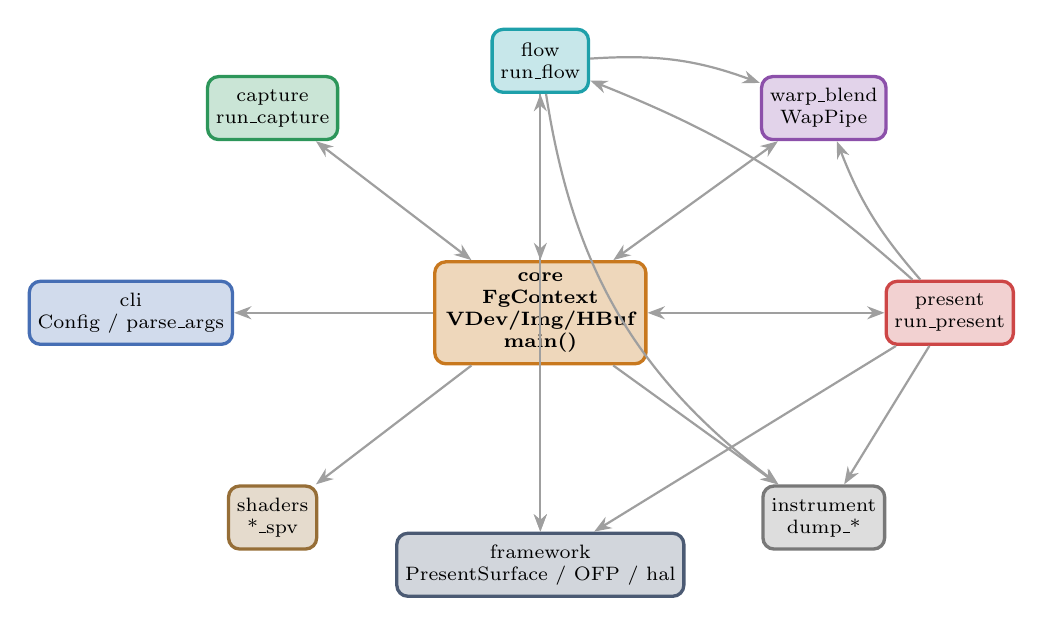
\begin{tikzpicture}[scale=1.0]
  % central hub
  \node[hub, fill=coreCol!30, draw=coreCol] (core) at (0,0) {core\\\scriptsize FgContext\\\scriptsize VDev/Img/HBuf\\\scriptsize main()};
  % satellites
  \node[mod, fill=cliCol!25,  draw=cliCol]  (cli)   at (-5.2,0)   {cli\\\scriptsize Config / parse\_args};
  \node[mod, fill=capCol!25,  draw=capCol]  (cap)   at (-3.4,2.6) {capture\\\scriptsize run\_capture};
  \node[mod, fill=flowCol!25, draw=flowCol] (flow)  at (0,3.2)    {flow\\\scriptsize run\_flow};
  \node[mod, fill=warpCol!25, draw=warpCol] (warp)  at (3.6,2.6)  {warp\_blend\\\scriptsize WapPipe};
  \node[mod, fill=presCol!25, draw=presCol] (pres)  at (5.2,0)    {present\\\scriptsize run\_present};
  \node[mod, fill=instCol!25, draw=instCol] (inst)  at (3.6,-2.6) {instrument\\\scriptsize dump\_*};
  \node[mod, fill=fwCol!25,   draw=fwCol]   (fw)    at (0,-3.2)   {framework\\\scriptsize PresentSurface / OFP / hal};
  \node[mod, fill=shCol!25,   draw=shCol]   (sh)    at (-3.4,-2.6){shaders\\\scriptsize *\_spv};

  % core <-> workers (bidir: main includes *.hpp; *.cpp include fg_context/device/vk_util)
  \draw[bidir] (core) -- (cap);
  \draw[bidir] (core) -- (flow);
  \draw[bidir] (core) -- (warp);
  \draw[bidir] (core) -- (pres);
  % core -> leaves
  \draw[dep] (core) -- (cli);
  \draw[dep] (core) -- (fw);
  \draw[dep] (core) -- (sh);
  \draw[dep] (core) -- (inst);
  % flow deps
  \draw[dep] (flow) -- (fw);
  \draw[dep] (flow) to[bend left=12] (warp);
  \draw[dep] (flow) to[bend right=22] (inst);
  % present deps
  \draw[dep] (pres) -- (fw);
  \draw[dep] (pres) to[bend left=10] (warp);
  \draw[dep] (pres) to[bend right=10] (flow);
  \draw[dep] (pres) -- (inst);
\end{tikzpicture}

\vspace{2pt}
{\tiny \textcolor{gray}{\textbf{Flecha llena} = depende-de / \#include \quad\textbar\quad \textbf{Doble cabeza} = \texttt{main.cpp} incluye el \texttt{.hpp} \emph{y} el \texttt{.cpp} incluye \texttt{fg\_context/device/vk\_util}. \quad core/FgContext = el hub.}}
\end{frame}

% ===================== DATAFLOW C/F/P (TikZ) =====================
\begin{frame}{Flujo de datos C\,/\,F\,/\,P (per-frame, izquierda\arr{}derecha)}
\centering
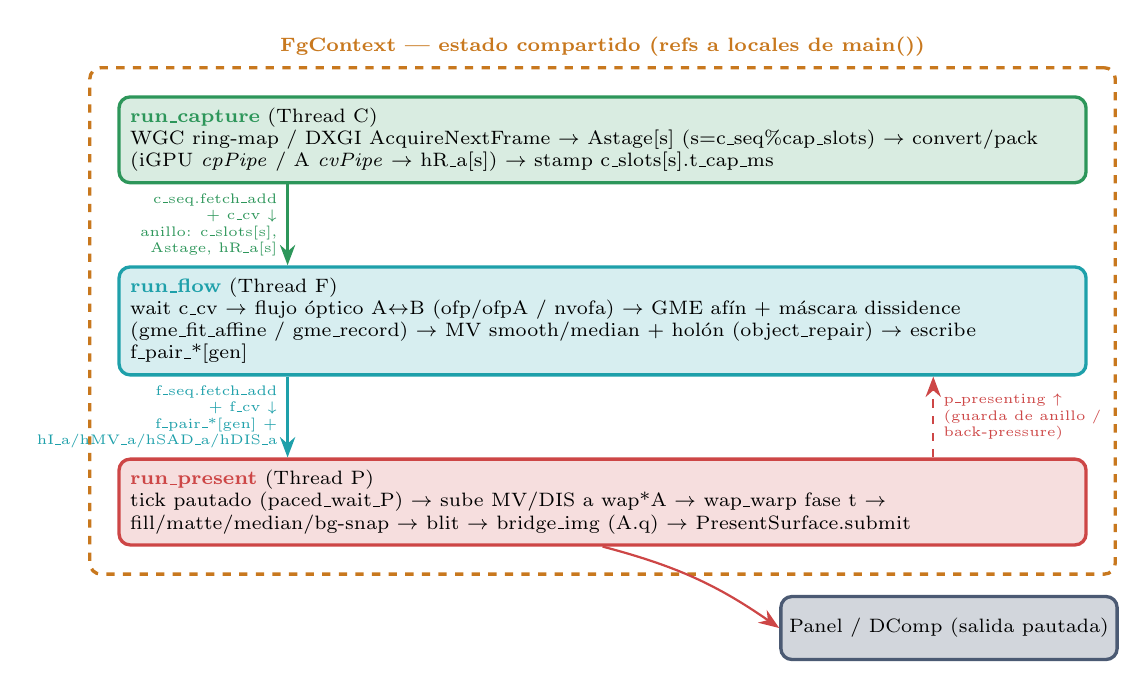
\begin{tikzpicture}
  \node[lane, fill=capCol!18, draw=capCol] (laneC) at (0,2.3)
    {\Lcap{run\_capture} (Thread C)\\
     WGC ring-map / DXGI AcquireNextFrame $\to$ Astage[s] (s$=$c\_seq\%cap\_slots) $\to$
     convert/pack (iGPU \emph{cpPipe} / A \emph{cvPipe} $\to$ hR\_a[s]) $\to$ stamp c\_slots[s].t\_cap\_ms};
  \node[lane, fill=flowCol!18, draw=flowCol] (laneF) at (0,0.0)
    {\Lflow{run\_flow} (Thread F)\\
     wait c\_cv $\to$ flujo \'optico A$\leftrightarrow$B (ofp/ofpA / nvofa) $\to$ GME af\'in + m\'ascara
     dissidence (gme\_fit\_affine / gme\_record) $\to$ MV smooth/median + hol\'on (object\_repair)
     $\to$ escribe f\_pair\_*[gen]};
  \node[lane, fill=presCol!18, draw=presCol] (laneP) at (0,-2.3)
    {\Lpres{run\_present} (Thread P)\\
     tick pautado (paced\_wait\_P) $\to$ sube MV/DIS a wap*A $\to$ wap\_warp fase t $\to$
     fill/matte/median/bg-snap $\to$ blit $\to$ bridge\_img (A.q) $\to$ PresentSurface.submit};
  \node[mod, fill=fwCol!25, draw=fwCol] (panel) at (4.4,-3.9) {\scriptsize Panel / DComp (salida pautada)};

  % C -> F (left)
  \draw[chan, capCol] ([xshift=-40mm]laneC.south) -- node[left, font=\tiny, align=right]
      {c\_seq.fetch\_add\\ + c\_cv $\downarrow$\\ anillo: c\_slots[s],\\ Astage, hR\_a[s]}
      ([xshift=-40mm]laneF.north);
  % F -> P (left)
  \draw[chan, flowCol] ([xshift=-40mm]laneF.south) -- node[left, font=\tiny, align=right]
      {f\_seq.fetch\_add\\ + f\_cv $\downarrow$\\ f\_pair\_*[gen] +\\ hI\_a/hMV\_a/hSAD\_a/hDIS\_a}
      ([xshift=-40mm]laneP.north);
  % P -> F back-edge (right, dashed)
  \draw[back] ([xshift=42mm]laneP.north) -- node[right, font=\tiny, align=left]
      {p\_presenting $\uparrow$\\ (guarda de anillo /\\ back-pressure)}
      ([xshift=42mm]laneF.south);
  % P -> panel
  \draw[chan, presCol] (laneP.south) to[bend left=10] (panel.west);

  \begin{scope}[on background layer]
    \node[fit=(laneC)(laneF)(laneP), draw=coreCol, very thick, dashed,
          rounded corners, inner sep=3.5mm,
          label={[coreCol,font=\scriptsize\bfseries]above:FgContext --- estado compartido (refs a locales de main())}] {};
  \end{scope}
\end{tikzpicture}
\end{frame}

% ===================== TABLA POR MODULO =====================
\begin{frame}[allowframebreaks]{Tabla por m\'odulo}
\scriptsize
\setlength{\tabcolsep}{3pt}
\renewcommand{\arraystretch}{1.12}
\begin{longtable}{p{1.35cm} p{2.85cm} p{2.35cm} p{2.65cm} p{2.55cm}}
\toprule
\textbf{M\'odulo} & \textbf{Provee (s\'imbolos clave)} & \textbf{Depende de} & \textbf{Campos FgContext} & \textbf{Rol} \\
\midrule
\endfirsthead
\toprule
\textbf{M\'odulo} & \textbf{Provee} & \textbf{Depende de} & \textbf{Campos FgContext} & \textbf{Rol} \\
\midrule
\endhead
\bottomrule
\endfoot

\Lcli{cli} &
\texttt{Config}; enums \texttt{CaptureApi}/\texttt{FgGpu}/\texttt{ConvertGpu}/\texttt{OutputClock}; \texttt{kMaxInterp}/\texttt{kAutoNMax}; \texttt{print\_help}, \texttt{parse\_args}, \texttt{parse\_extra} &
solo stdlib (\texttt{cli/cli.hpp}) &
ninguno &
Hoja CLI: define \texttt{Config} + parser; no toca FgContext/threads. \\

\Lcore{core} &
\texttt{FgContext}, \texttt{RealSlot}, \texttt{VDev}, \texttt{Img}, \texttt{HBuf}; \texttt{vdev\_create}, \texttt{img\_create}, \texttt{hbuf\_import}, \texttt{submit\_wait(\_q2)}, \texttt{oneshot}, \texttt{route\_for}, \texttt{vk\_live}, globals (\texttt{g\_quit}...), \texttt{main()} &
cli, capture, flow, warp\_blend, present, instrument, framework, shaders &
\textbf{define TODOS} (\texttt{c\_seq}, \texttt{f\_seq}, \texttt{p\_presenting}, \texttt{f\_pair\_*}, \texttt{c\_slots}, pacing) &
Substrato + orquestador: aggregate-init \texttt{ctx} + spawn/join de los 3 threads. \\

\Lcap{capture} &
\texttt{run\_capture}; \texttt{D3D}, \texttt{OutInfo}, \texttt{ConvPackPipe}, \texttt{UnpackPipe}; \texttt{d3d\_init/shutdown/staging(\_on)}, \texttt{cpipe\_create}, \texttt{unpipe\_create}, \texttt{find\_window\_by\_substr} &
core (device/vk\_util/fg\_context), \texttt{vulkan.h} &
\textbf{escribe} \texttt{c\_seq}, \texttt{c\_cv}, \texttt{c\_slots[s].t\_cap\_ms}; \textbf{lee} \texttt{cfg}, \texttt{d}, \texttt{wgc\_ctx}, \texttt{Astage}, \texttt{A}/\texttt{G} &
Thread C: captura WGC/DDA $\to$ convert/pack $\to$ publica \texttt{c\_seq}. \\

\Lflow{flow} &
\texttt{run\_flow}; \texttt{NvofaProvider}, \texttt{GmePipe}, \texttt{MvSmoothPipe}, \texttt{MedianPipe}; \texttt{gme\_fit\_affine}, \texttt{nvofa\_*}, \texttt{gme\_*}, \texttt{object\_repair}, \texttt{mem\_advect/merge/refresh}, \texttt{kGenRing} &
core; framework (\texttt{OpticalFlowPipeline}); warp\_blend (stats); instrument &
\textbf{lee} \texttt{c\_seq}/\texttt{c\_slots}, \texttt{p\_presenting} (back-edge); \textbf{escribe} \texttt{f\_seq}, \texttt{f\_pair\_*}, bridges \texttt{hostMV}/\texttt{hostDIS}... &
Thread F: flujo \'optico + GME + hol\'on $\to$ publica pares v\'ia \texttt{f\_seq}. \\

\Lwarp{warp\_blend} &
\texttt{WapPipe} (\texttt{wap\_create}), \texttt{FieldPipe} (\texttt{fpipe\_*}), \texttt{FillPipe} (\texttt{fillpipe\_*}); \texttt{matte\_mass\_count}, \texttt{gme\_dispct\_from\_mask} &
core (\texttt{device.hpp}), \texttt{vulkan.h} &
ninguno (biblioteca stateless de f\'abricas) &
F\'abricas de pipelines warp/blend/quality; el \emph{dispatch} vive en \texttt{run\_present}. \\

\Lpres{present} &
\texttt{run\_present}; \texttt{UpPipe} (\texttt{up\_create}), \texttt{OverlayFpsPC}, \texttt{BridgeSlot}; \texttt{wap\_upload}, \texttt{wap\_warp\_present}, \texttt{bridge\_present(\_src)}, \texttt{paced\_wait\_P}, \texttt{rfp\_present} &
core; framework (\texttt{PresentSurface}, \texttt{hal}); warp\_blend; flow; instrument &
\textbf{lee} \texttt{f\_seq}/\texttt{f\_pair\_*}/\texttt{c\_seq}; \textbf{escribe} \texttt{total\_frames}, \texttt{present\_cost\_us}; \texttt{bridge\_img}/\texttt{wapPipeA}/\texttt{A.qT} &
Thread P: selecciona fase, warp/upscale/blit $\to$ \texttt{PresentSurface.submit}. \\

\Linst{instrument} &
\texttt{dump\_bmp}, \texttt{dump\_rgba} &
solo \texttt{instrument.hpp} &
ninguno &
Volcado de frames (BMP/RGBA), sin acoplamiento a pipeline/FgContext. \\

\Lfw{framework} &
\texttt{PresentSurface} (\texttt{create}/\texttt{submit}/\texttt{device\_lost}), \texttt{OpticalFlowPipeline} (\texttt{init}/\texttt{record\_optical\_flow}/\texttt{record\_warp\_only}), \texttt{Error}/\texttt{ErrorCode}, \texttt{HardwareTopology}, \texttt{hal} (f16, cpu\_wait, atomics, TSC, SIMD), \texttt{schema} &
externo: \texttt{vulkan.h}, Win32/D3D11/DXGI/DComp; SPIR-V \texttt{optical\_flow\_*} &
N/A (FgContext es app-local; provee las primitivas que lo rodean) &
Substrato vendido: P-stage + F-engine + hal/topology/schema. \\

\Lshd{shaders} &
\texttt{*\_spv.hpp}: \texttt{hdr\_convert}, \texttt{igpu\_convert\_pack}, \texttt{unpack\_packed}, \texttt{igpu\_field}, \texttt{wap\_warp}, \texttt{wap\_fill}, \texttt{mv\_smooth}, \texttt{mv\_median}, \texttt{nvofa\_convert}, \texttt{gme\_reduce/solve/dissidence}, \texttt{upscale\_bilinear/lanczos}, \texttt{overlay\_fps} &
nada (bytecode); incluido por \texttt{core/main.cpp} &
ninguno &
Bytecode SPIR-V de los pipelines compute. \\

\end{longtable}
\end{frame}

% ===================== QUE AGREGA QUE, EN QUE CAPA =====================
\begin{frame}[allowframebreaks]{Qu\'e agrega qu\'e, en qu\'e capa (s\'imbolos + l\'inea, structs, shaders)}
\scriptsize
\setlength{\tabcolsep}{3pt}
\renewcommand{\arraystretch}{1.12}
\begin{longtable}{p{1.35cm} p{4.6cm} p{2.5cm} p{3.1cm}}
\toprule
\textbf{Capa} & \textbf{S\'imbolos clave (archivo:l\'inea nuevos)} & \textbf{Pipelines/structs propios} & \textbf{Shaders usados} \\
\midrule
\endfirsthead
\toprule
\textbf{Capa} & \textbf{S\'imbolos (archivo:l\'inea)} & \textbf{Pipelines/structs} & \textbf{Shaders} \\
\midrule
\endhead
\bottomrule
\endfoot

\Lcli{cli} &
\texttt{Config}@cli.hpp:15; \texttt{parse\_args}@cli.cpp:115; \texttt{parse\_extra}@cli.cpp:124; \texttt{print\_help}@cli.cpp:8; \texttt{kMaxInterp}@cli.hpp:853 &
\texttt{Config} POD + enums &
--- \\

\Lcore{core} &
\texttt{FgContext}@fg\_context.hpp:37; \texttt{RealSlot}@:35; \texttt{main}@main.cpp:167 (ctx@2549, spawn@2797--2799, join@2806--2809); \texttt{VDev}@device.hpp:20; \texttt{vdev\_create}@device.cpp:9; \texttt{route\_for}@vk\_util.cpp:7; \texttt{vk\_live}@globals.cpp:13 &
\texttt{VDev}/\texttt{Img}/\texttt{HBuf}, \texttt{FgContext} &
embebe TODOS los \texttt{*\_spv} (main.cpp) \\

\Lcap{capture} &
\texttt{run\_capture}@capture.cpp:120; \texttt{d3d\_init}@:13; \texttt{cpipe\_create}@:69; \texttt{unpipe\_create}@:93 &
\texttt{D3D}, \texttt{ConvPackPipe}, \texttt{UnpackPipe} &
\texttt{igpu\_convert\_pack}, \texttt{unpack\_packed}, \texttt{hdr\_convert} \\

\Lflow{flow} &
\texttt{run\_flow}@flow.cpp:481; \texttt{gme\_fit\_affine}@:49; \texttt{nvofa\_create}@:166; \texttt{gme\_record}@:404; \texttt{object\_repair}@:887; \texttt{mem\_refresh}@:1329; \texttt{kGenRing}@flow.hpp:27 &
\texttt{NvofaProvider}, \texttt{GmePipe}, \texttt{MvSmoothPipe}, \texttt{MedianPipe} &
\texttt{nvofa\_convert}, \texttt{gme\_reduce/solve/dissidence}, \texttt{mv\_smooth}, \texttt{mv\_median} \\

\Lwarp{warp\_blend} &
\texttt{wap\_create}@warp\_blend.cpp:153; \texttt{fpipe\_create}@:37; \texttt{fillpipe\_create}@:61; \texttt{matte\_mass\_count}@:14 &
\texttt{WapPipe}, \texttt{FieldPipe}, \texttt{FillPipe} &
\texttt{wap\_warp}, \texttt{wap\_fill}, \texttt{igpu\_field} \\

\Lpres{present} &
\texttt{run\_present}@present.cpp:57; \texttt{wap\_upload}@:694; \texttt{wap\_warp\_present}@:860; \texttt{bridge\_present\_src}@:629; \texttt{paced\_wait\_P}@:509; loop present@:1530; \texttt{up\_create}@:34 &
\texttt{UpPipe}, \texttt{BridgeSlot} &
\texttt{upscale\_bilinear/lanczos}, \texttt{unpack\_packed}, \texttt{overlay\_fps} \\

\Linst{instrument} &
\texttt{dump\_bmp}@instrument.cpp:11; \texttt{dump\_rgba}@:32 &
--- &
--- \\

\Lfw{framework} &
\texttt{PresentSurface}@:139 (\texttt{create}@:145 / \texttt{submit}@:159); \texttt{OpticalFlowPipeline}@:34 (\texttt{init}@:163 / \texttt{record\_optical\_flow}@:217); \texttt{Error}@:58; \texttt{HardwareTopology}@:111 (\texttt{probe}@:128); \texttt{f16\_to\_f32}@Simd.hpp:195 &
\texttt{PresentSurface}, \texttt{OpticalFlowPipeline} &
\texttt{optical\_flow\_\{pyr\_down,hier\_match,hier\_match\_fg,warp,affine\_fit\}} \\

\end{longtable}
\end{frame}

% ===================== CONEXIONES POR ELEMENTO =====================
\begin{frame}[allowframebreaks]{Conexiones por elemento (si toco X, qu\'e se ve afectado)}
\scriptsize
\setlength{\tabcolsep}{3pt}
\renewcommand{\arraystretch}{1.18}
\begin{longtable}{p{2.2cm} p{5.0cm} p{4.6cm}}
\toprule
\textbf{Elemento} & \textbf{Depende de} & \textbf{Lo usan (ripple)} \\
\midrule
\endfirsthead
\toprule
\textbf{Elemento} & \textbf{Depende de} & \textbf{Lo usan (ripple)} \\
\midrule
\endhead
\bottomrule
\endfoot

\Lcore{FgContext} &
tipos \texttt{VDev}/\texttt{Img}/\texttt{HBuf} (core), \texttt{Config} (cli); refs a locales de \texttt{main()} &
\textbf{los 3 threads} (\texttt{run\_capture}/\texttt{run\_flow}/\texttt{run\_present} aliasen sus campos); \texttt{main} aggregate-init @2549. Tocar un campo $\Rightarrow$ re-mira C, F y P. \\

\Lcap{run\_capture} &
\texttt{D3D}/\texttt{WgcCtx}, \texttt{VDev} A/G, \texttt{Astage}, \texttt{cfg}, \texttt{img\_barrier}/\texttt{full\_bic}/\texttt{submit\_wait}, MMCSS/pin &
\texttt{run\_flow} (consume \texttt{c\_seq} + el anillo); \texttt{main} (spawn) \\

\Lflow{run\_flow} &
\texttt{FgContext}, \texttt{OpticalFlowPipeline} (ofp/ofpA), \texttt{NvofaProvider}, \texttt{GmePipe}, \texttt{MvSmoothPipe}, \texttt{MedianPipe}, \texttt{gme\_fit\_affine}, \texttt{ra::decode\_f16}, stats de warp\_blend &
\texttt{run\_present} (consume \texttt{f\_seq} + \texttt{f\_pair\_*}); lee \texttt{p\_presenting} de P; \texttt{main} (spawn) \\

\Lpres{run\_present} &
\texttt{FgContext}, \texttt{PresentSurface}, \texttt{WapPipe} (wapPipeA), \texttt{UpPipe}, \texttt{MedianPipe}, \texttt{hal::cpu\_wait\_for\_ns}, \texttt{TelemetryCsv} &
panel/DComp (salida); \texttt{run\_flow} lee \texttt{p\_presenting} (back-edge); \texttt{main} (spawn) \\

\Lfw{OpticalFlowPipeline} &
\texttt{hal}, \texttt{vulkan.h}, SPIR-V \texttt{optical\_flow\_*} &
\texttt{run\_flow} (ofp/ofpA: \texttt{record\_optical\_flow} / \texttt{record\_warp\_only}) \\

\Lwarp{WapPipe} &
\texttt{VDev}, SPIR-V \texttt{wap\_warp}, 14 bindings + push 212B (53 floats) &
\texttt{run\_present} (\texttt{wap\_upload} + \texttt{wap\_warp\_present}) \\

\Lcore{F\'abricas de pipelines} &
\texttt{VDev} + llamadas \texttt{vk*Create*} + SPIR-V (\texttt{vdev}/\texttt{img}/\texttt{hbuf}/\texttt{cpipe}/\texttt{unpipe}/\texttt{wap}/\texttt{fpipe}/\texttt{fillpipe}/\texttt{up}/\texttt{gme}/\texttt{mvsm}/\texttt{med}/\texttt{nvofa}) &
\texttt{main} las construye en init; los threads despachan. Tocar una firma $\Rightarrow$ re-mira init + el thread due\~no. \\

\end{longtable}
\end{frame}

% ===================== COMO USAR ESTE MAPA =====================
\begin{frame}{C\'omo usar este mapa}
\small
\textbf{Para tocar X, ve a Y:}
\begin{itemize}\setlength\itemsep{2pt}
  \item Un flag CLI \arr{} \Lcli{cli/cli.cpp} (\texttt{parse\_args} / \texttt{parse\_extra}) + \texttt{Config}@cli.hpp:15
  \item El contrato C/F/P \arr{} \Lcore{core/fg\_context.hpp} (\texttt{FgContext}) --- re-mira los \textbf{3 threads}
  \item La captura \arr{} \Lcap{capture/capture.cpp} (\texttt{run\_capture})
  \item El flujo/hol\'on \arr{} \Lflow{flow/flow.cpp} (\texttt{run\_flow})
  \item El warp/blend \arr{} \Lwarp{warp\_blend} (f\'abrica) + \Lpres{present/present.cpp} (dispatch real)
  \item El present/pacing \arr{} \Lpres{present/present.cpp} (\texttt{run\_present})
\end{itemize}
\vspace{4pt}
\textbf{Las flechas del DAG = qu\'e se ve afectado:} si tocas un nodo, lo que \emph{apunta hacia \'el}
(sus dependientes) puede romperse. \Lcore{FgContext} es el hub --- un cambio ah\'i toca C, F y P a la vez.
Las f\'abricas son stateless: cambiar una firma re-mira el init de \texttt{main} m\'as su thread due\~no.
\end{frame}

\end{document}
